\documentclass[11pt]{article}

% ---------- Core packages ----------
\usepackage[T1]{fontenc}
\usepackage[margin=1in,top=1.15in,bottom=1.15in]{geometry}
\usepackage{graphicx}
\usepackage{tikz}
\usetikzlibrary{arrows.meta, positioning, fit, backgrounds}
\usepackage{booktabs}
\usepackage{tabularx}
\usepackage{float}
\usepackage{colortbl}
\usepackage{array}
\usepackage{xcolor}
\usepackage{enumitem}
\usepackage{fancyhdr}
\usepackage{titlesec}
\usepackage{titletoc}
\usepackage{caption}
\usepackage{parskip}
\usepackage{amsmath}
\usepackage[hidelinks]{hyperref}
\usepackage{graphicx}
\usepackage{float}


% ---------- Palette ----------
\definecolor{navy}{RGB}{22,45,82}
\definecolor{accent}{RGB}{41,98,168}
\definecolor{accentlight}{RGB}{223,235,247}
\definecolor{rowalt}{RGB}{244,247,251}
\definecolor{rulegray}{RGB}{200,205,212}
\definecolor{bodytext}{RGB}{35,38,42}

% diagram palette
\definecolor{storageFill}{RGB}{219,232,250} \definecolor{storageLine}{RGB}{66,113,181}
\definecolor{streamFill}{RGB}{252,228,209}  \definecolor{streamLine}{RGB}{214,120,44}
\definecolor{computeFill}{RGB}{224,240,213} \definecolor{computeLine}{RGB}{101,157,73}
\definecolor{dbFill}{RGB}{237,224,247}      \definecolor{dbLine}{RGB}{140,90,180}
\definecolor{webFill}{RGB}{255,242,204}     \definecolor{webLine}{RGB}{176,140,10}

\color{bodytext}

% ---------- Section styling ----------
\titleformat{\section}
  {\Large\bfseries\color{navy}}
  {\colorbox{navy}{\makebox[1.6em][c]{\color{white}\thesection}}}
  {0.6em}{}
\titlespacing*{\section}{0pt}{1.6em}{0.9em}

\titleformat{\subsection}
  {\large\bfseries\color{accent}}
  {\thesubsection}{0.6em}{}
\titlespacing*{\subsection}{0pt}{1.1em}{0.5em}

\renewcommand{\contentsname}{\color{navy}Table of Contents}
\titlecontents{section}[0em]{\vspace{2pt}\bfseries}
  {\contentsmargin{0pt}\color{navy}\thecontentslabel.\enspace}{}
  {\hfill\thecontentspage}
\titlecontents{subsection}[1.6em]{\vspace{1pt}}
  {\contentsmargin{0pt}\thecontentslabel\enspace}{}
  {\titlerule*[6pt]{.}\thecontentspage}

% ---------- Header / footer ----------
\pagestyle{fancy}
\setlength{\headheight}{22pt}
\fancyhf{}
\renewcommand{\headrulewidth}{0.6pt}
\renewcommand{\headrule}{\hbox to\headwidth{\color{rulegray}\leaders\hrule height \headrulewidth\hfill}}
\fancyhead[L]{\small\color{navy}\textsc{Sales Forecasting Pipeline}}
\fancyhead[R]{\small\color{navy}\thepage}
\renewcommand{\footrulewidth}{0pt}
\fancyfoot[C]{\small\color{rulegray}Big Data Essentials Course Project}

\fancypagestyle{plain}{%
  \fancyhf{}
  \fancyfoot[C]{\small\color{rulegray}Big Data Essentials Course Project}
  \renewcommand{\headrulewidth}{0pt}
}

\setlength{\parskip}{0.55em}
\setlength{\parindent}{0pt}

% helper for step headings
\newcommand{\stephead}[2]{\par\vspace{0.4em}\noindent{\color{white}\colorbox{accent}{\textbf{\,Step #1\,}}}\ \textbf{#2}\par\vspace{0.15em}}

% metric-style callout box
\newcommand{\statbox}[3]{%
  \begin{minipage}[t]{0.315\textwidth}
    \centering
    \begin{tikzpicture}
      \node[fill=accentlight, rounded corners=3pt, inner sep=8pt, text width=0.82\linewidth, align=center]
        {\textbf{\color{navy}#1}\\[3pt]{\large\bfseries #2}\\[2pt]{\small #3}};
    \end{tikzpicture}
  \end{minipage}%
}

\begin{document}

% ==================== TITLE PAGE ====================
\begin{titlepage}
\newgeometry{margin=0in}
\begin{tikzpicture}[remember picture, overlay]
  \fill[navy] (current page.north west) rectangle ([yshift=-3.6cm]current page.north east);
  \fill[accent] ([yshift=-3.6cm]current page.north west) rectangle ([yshift=-3.78cm]current page.north east);
  \fill[navy] (current page.south west) rectangle ([yshift=0.9cm]current page.south east);
\end{tikzpicture}

\vspace*{0.55cm}
\hspace{1.6cm}{\color{white}\large\textsc{Big Data Essentials Course Project, Report For Final Exam}}

\vspace{3.6cm}
\begin{center}
    \fontsize{24pt}{30pt}\selectfont
   \MakeUppercase{ADVENTIST UNIVERSITY OF CENTRAL AFRICA}
\end{center}

\begin{center}
{\huge\bfseries\color{navy} Real-Time Sales Forecasting for a\\[3pt] Multi-Store Retail Chain}

\vspace{0.7cm}
{\Large\itshape\color{accent} Integrating HDFS, Kafka, PySpark, MLlib, MySQL, and Django}

\Large\textbf{Prepared by group (9) members}\\[10pt]
\begin{center}
\begin{tikzpicture}
\node[draw=rulegray, thick, rounded corners=4pt, inner sep=16pt] {%
    \begin{tabular}{ll}
        \textbf{Student ID} & \textbf{Names} \\[5pt]
        101215 & Richard Mwenedata \\
        101216 & Pascal Kabagema \\
        101207 & Denyse Mutoni \\
        101248 & Salome Mukarugaba \\
        101188 & Daniel Urimubenshi \\
 \end{tabular}};
\end{tikzpicture}
\end{center}
\vspace{1cm}
{\Large\color{navy}\textbf{Case Study: Sales Forecasting}}\\[6pt]
\begin{tikzpicture}
\node[draw=rulegray, thick, rounded corners=4pt, inner sep=16pt] {%
\begin{tabular}{@{}ll@{}}
\textbf{\color{navy}Course:} & Big Data Essentials \\[6pt]
\textbf{\color{navy}Lecturer:} & Dr.\ Kundan Kumar \\[6pt]
\textbf{\color{navy}Environment:} & Windows 11 \\[6pt]
\textbf{\color{navy}Date:} & September 2026 \\
\end{tabular}};
\end{tikzpicture}
\end{center}
\begin{center}
 \fontsize{14pt}{20pt}\selectfont
{\Large \textcolor{blue}{\href{https://github.com/Rich-code01/ecommerce_final_project.git}{This project can be found on GitHub, click this link}}}\\[0.5cm]
\end{center}
\vfill
\hspace{1.6cm}{\color{white}\footnotesize Pipeline: HDFS $\rightarrow$ Kafka $\rightarrow$ PySpark $\rightarrow$ MLlib $\rightarrow$ MySQL $\rightarrow$ Django}
\vspace{0.5cm}

\restoregeometry
\end{titlepage}

% ==================== TABLE OF CONTENTS ====================
\tableofcontents
\thispagestyle{plain}
\newpage
% ==================== ABSTRACT ====================
\thispagestyle{plain}
\begin{center}
{\section{\large\bfseries\color{navy} Abstract}}
\end{center}

\noindent
Retail organizations increasingly rely on data-driven forecasting to anticipate demand, manage inventory, and respond to real-time sales patterns. This project presents the design and implementation of an end-to-end Big Data pipeline for real-time sales forecasting, built for a simulated multi-store, multi-region retail chain, and developed as a course project for Big Data Essentials. The system integrates six core technologies. Hadoop Distributed File System (HDFS), Apache Kafka, Apache Spark (batch and Structured Streaming), Spark MLlib, MySQL, and Django into a single working architecture that spans distributed storage, real-time message streaming, distributed processing, machine learning, relational persistence, and web-based visualization, all deployed on a Windows 11 workstation.

\vspace{0.3cm}
\noindent
The pipeline follows two parallel data paths that converge at a shared presentation layer. In the batch training path, a synthetically generated dataset of 17.5 million transaction records (1.12 GB), covering 25 stores across 5 regions, 200 products, and 8 categories over five years (2022-2026), is stored in HDFS. A PySpark batch job aggregates this data to daily granularity, engineers ten time-series and calendar-based features, and trains a Random Forest Regressor to forecast daily revenue, writing the resulting predictions to MySQL via JDBC. In the real-time streaming path, a Kafka producer replays the same dataset as a simulated point-of-sale feed, which a PySpark Structured Streaming consumer ingests, parses, and aggregates into live region-and-category-level totals, persisting these to MySQL through a \texttt{foreachBatch} sink. A Django web application then serves both the historical predictions and the live streaming data through four dashboard views. Overview, Predictions, Charts, and Live with the Live view polling a JSON endpoint every 2.5 seconds to reflect new data without a page reload.

\vspace{0.3cm}
\noindent
The trained forecasting model was evaluated on a time-based, held-out test set of the most recent 180 days, avoiding the data leakage risk of random splitting in a time-series context. The model achieved strong predictive accuracy, with an R\textsuperscript{2} of 0.9969, an RMSE of approximately 233{,}398, and an MAE of approximately 177{,}180 revenue units. Feature importance analysis showed that daily units sold was by far the dominant predictor (50.7\% importance), followed collectively by calendar-based seasonality features month, weekend, and holiday-season indicators which together validate the deliberate demand patterns embedded in the synthetic dataset. Lag-based features, including previous-day revenue and a 7-day rolling average, contributed modestly, indicating some residual short-term momentum in the data beyond same-day attributes.

\vspace{0.3cm}
\noindent
This work demonstrates that a fully integrated Big Data pipeline combining distributed storage, real-time streaming, distributed machine learning, and interactive visualization can be implemented and verified end-to-end on commodity hardware, with the live dashboard reflecting streaming updates within seconds of ingestion. The results confirm both the technical feasibility of the architecture and the interpretability of the underlying forecasting model, offering a template for similar real-time analytics systems in retail and adjacent domains.

\vspace{0.5cm}
\noindent
\textbf{\color{navy}Keywords:} Big Data, Real-Time Streaming, Apache Kafka, Apache Spark, Structured Streaming, Machine Learning, Sales Forecasting, Random Forest, MySQL, Django

\newpage
% ==================== 1. PROJECT OVERVIEW ====================
\section{Project Overview}

This project implements an end-to-end Big Data pipeline for real-time sales forecasting, developed to satisfy the Big Data Essentials course project requirements. The system integrates distributed storage, real-time message streaming, distributed data processing, machine learning, relational storage, and web-based visualization into a single working pipeline, running entirely on a Windows 11 workstation.

The chosen case study is Sales Forecasting for a simulated multi-store, multi-region retail chain. The objective is to predict daily total revenue using historical transaction patterns, seasonal effects, and real-time incoming transaction data.

\subsection{Objectives}

\begin{itemize}[leftmargin=1.4em, itemsep=2pt]
    \item Stream simulated real-time retail transactions using Apache Kafka, sourced from a dataset stored in HDFS.
    \item Process the streaming data in real time using PySpark Structured Streaming, producing both raw record views and live aggregated totals.
    \item Engineer time-series features from historical transaction data and train a machine learning model using Spark MLlib to forecast daily revenue.
    \item Persist both batch predictions and live streaming aggregates into a MySQL relational database.
    \item Build a Django web dashboard to visualize historical predictions, model performance, and the live data stream.
\end{itemize}

\subsection{Case Study Description}

The dataset simulates five years (2022-2026) of retail transactions across 25 stores in 5 regions, covering 200 products across 8 categories. Each transaction record includes the date, store, region, product, category, units sold, unit price, promotion flag, discount percentage, and resulting sales amount. Realistic patterns are embedded in the data generation process, including weekday/weekend demand variation, a November--December holiday sales spike, and promotional discount effects.

\vspace{0.3em}
\noindent
\statbox{Scale}{17.5M rows}{transactions generated}\hfill
\statbox{Coverage}{25 / 5 / 200}{stores / regions / products}\hfill
\statbox{Span}{5 years}{2022 - 2026}

\vspace{0.6em}

% ==================== 2. SYSTEM ARCHITECTURE ====================
\section{System Architecture}

The system is composed of two parallel data paths that converge at the dashboard layer: a batch training path (historical data $\rightarrow$ trained model $\rightarrow$ stored predictions) and a real-time streaming path (live transactions $\rightarrow$ streaming aggregation $\rightarrow$ live dashboard updates). Figure~\ref{fig:architecture} illustrates the full architecture.

\begin{figure}[H]
\centering
\resizebox{\textwidth}{!}{%
\begin{tikzpicture}[
  font=\sffamily\footnotesize,
  box/.style={draw, rounded corners=3pt, thick, align=center, minimum height=1.7cm, text width=3.0cm, inner sep=5pt},
  storage/.style={box, fill=storageFill, draw=storageLine},
  stream/.style={box, fill=streamFill, draw=streamLine},
  compute/.style={box, fill=computeFill, draw=computeLine},
  db/.style={box, fill=dbFill, draw=dbLine},
  web/.style={box, fill=webFill, draw=webLine, text width=15.4cm, minimum height=1.9cm},
  arr/.style={-{Latex[length=2.4mm]}, thick, draw=gray!65},
  lbl/.style={font=\sffamily\scriptsize, fill=white, inner sep=1pt}
]

% column x-positions: 0 / 4.6 / 9.2 / 13.9 -- generous gaps for edge labels

% Row 1: batch path
\node[storage] (dataset) at (0,7.4)   {\textbf{Sales Dataset}\\17.5M rows, 1.12\,GB\\\texttt{\scriptsize generate\_sales\_}\\\texttt{\scriptsize data.py}};
\node[storage] (hdfs)    at (4.6,7.4) {\textbf{HDFS}\\Hadoop 3.3.6\\\texttt{\scriptsize /project/}\\\texttt{\scriptsize sales\_data}};
\node[compute] (batch)   at (9.2,7.4) {\textbf{PySpark Batch Job}\\\texttt{\scriptsize train\_and\_}\\\texttt{\scriptsize predict.py}\\(feature eng.\ + MLlib)};
\node[db]      (dbpred)  at (15.9,7.4){\textbf{MySQL}\\[2pt]\texttt{\scriptsize daily\_sales\_}\\\texttt{\scriptsize predictions}};

\draw[arr] (dataset) -- node[lbl, above]{upload} (hdfs);
\draw[arr] (hdfs) -- node[lbl, above]{read} (batch);
\draw[arr] (batch) -- node[lbl, above, text width=2.2cm, align=center]{write (JDBC)} (dbpred);

% Row 2: streaming path
\node[stream]  (producer)  at (0,3.9)   {\textbf{Kafka Producer}\\\texttt{\scriptsize kafka\_}\\\texttt{\scriptsize producer.py}\\(HDFS $\to$ Kafka)};
\node[stream]  (topic)     at (4.6,3.9) {\textbf{Kafka Topic}\\\texttt{\scriptsize sales-stream}\\(KRaft, 3.9.2)};
\node[compute] (streaming) at (9.2,3.9) {\textbf{PySpark Structured}\\\textbf{Streaming Consumer}\\(parse + aggregate)};
\node[db]      (dblive)    at (13.9,3.9){\textbf{MySQL}\\[2pt]\texttt{\tiny live\_region\_}\\\texttt{\tiny category\_totals}\\\texttt{\tiny live\_recent\_}\\\texttt{\tiny transactions}};

\draw[arr] (hdfs) -- (producer);
\draw[arr] (producer) -- node[lbl, above]{publish} (topic);
\draw[arr] (topic) -- node[lbl, above]{consume} (streaming);
\draw[arr] (streaming) -- node[lbl, above, text width=2.2cm, align=center]{write (JDBC)} (dblive);

% Console output
\node[compute, minimum height=1.3cm] (console) at (9.2,1.3) {\textbf{Console Output}\\(raw records + running totals)};
\draw[arr] (streaming) -- (console);

% Web dashboard
\node[web] (dashboard) at (9.95,-1.3) {\textbf{Django Web Dashboard}\\Overview \textbullet\ Predictions \textbullet\ Charts \textbullet\ Live\\(reads MySQL via \texttt{\scriptsize mysql-connector-python})};

\draw[arr] (dbpred.south) to[out=-95,in=90] (dashboard.north -| dbpred);
\draw[arr] (dblive.south) to[out=-95,in=90] (dashboard.north -| dblive);

% Title
\node[font=\sffamily\bfseries\Large, color=navy] at (6.95,8.7) {Real-Time Sales Forecasting Pipeline System Architecture};

% Legend
\begin{scope}[shift={(0,-3.6)}, every node/.style={font=\sffamily\footnotesize}]
\node[storage, minimum height=0.6cm, minimum width=0.6cm, text width=0.55cm] (l1) at (0,0) {};
\node[right=4pt of l1] (t1) {Storage};
\node[stream, minimum height=0.6cm, minimum width=0.6cm, text width=0.55cm, right=1.1cm of t1] (l2) {};
\node[right=4pt of l2] (t2) {Streaming};
\node[compute, minimum height=0.6cm, minimum width=0.6cm, text width=0.55cm, right=1.1cm of t2] (l3) {};
\node[right=4pt of l3] (t3) {Compute (Spark)};
\node[db, minimum height=0.6cm, minimum width=0.6cm, text width=0.55cm, right=1.1cm of t3] (l4) {};
\node[right=4pt of l4] (t4) {Database};
\node[web, minimum height=0.6cm, minimum width=0.6cm, text width=0.55cm, right=1.1cm of t4] (l5) {};
\node[right=4pt of l5] (t5) {Web / Dashboard};
\end{scope}

\end{tikzpicture}%
}
\caption{End-to-end system architecture}
\label{fig:architecture}
\end{figure}

\subsection{Batch Training Path}

The full transaction dataset (17.5 million records, 1.12 GB) is generated locally and uploaded to HDFS. A PySpark batch job reads this dataset from HDFS, aggregates it to daily granularity, engineers time-series features, trains a Random Forest Regressor via Spark MLlib, evaluates it on a held-out time window, and writes the resulting predictions to a MySQL table via JDBC.

\subsection{Real-Time Streaming Path}

A Kafka producer reads the same dataset from HDFS and publishes transaction records one at a time into a Kafka topic, simulating a live point-of-sale feed at a configurable rate. A PySpark Structured Streaming job subscribes to this topic, parses each JSON message, and maintains two continuously updated views: a raw record feed and a running total of revenue and units sold grouped by region and category. Both views are printed to the console and written to MySQL via a \texttt{foreachBatch} sink, making the live data available to the web dashboard.

\subsection{Presentation Layer}

A Django application serves four pages, all reading exclusively from MySQL: an Overview page with summary KPIs and model accuracy metrics; a paginated Predictions table; a Charts page with four visualizations of model performance; and a Live page that polls a JSON endpoint every 2.5 seconds to reflect the real-time streaming data, including a live/idle status indicator and flash notifications when new data arrives.

% ==================== 3. TECHNOLOGIES USED ====================
\section{Technologies Used}

The following table lists every core technology used in the project along with the exact version installed and verified during development.

\renewcommand{\arraystretch}{1.25}
\begin{table}[H]
\centering
\begin{tabularx}{\textwidth}{@{}>{\raggedright\arraybackslash}p{3.9cm}>{\raggedright\arraybackslash}p{3.6cm}>{\raggedright\arraybackslash}X@{}}
\toprule
\rowcolor{navy}\textcolor{white}{\textbf{Technology}} & \textcolor{white}{\textbf{Version}} & \textcolor{white}{\textbf{Role}} \\
\midrule
Java (Eclipse Temurin) & 11.0.32.101 & JVM runtime for Hadoop, Kafka, and Spark \\
\rowcolor{rowalt} Hadoop (HDFS) & 3.3.6 & Distributed storage for the source dataset \\
Apache Kafka & 3.9.2 (KRaft mode) & Real-time message streaming \\
\rowcolor{rowalt} Apache Spark & 3.5.9 (cluster) / PySpark 3.5.1 & Distributed batch and stream processing, MLlib \\
MySQL Server & 8.0 (custom port 3307) & Relational storage for predictions and live data \\
\rowcolor{rowalt} MySQL Connector/J & 26.7.0 & JDBC driver used by Spark to write to MySQL \\
Django & 6.1 & Web dashboard framework \\
\rowcolor{rowalt} Python & 3.14.7 & Primary scripting language \\
Chart.js & 4.4.1 (via CDN) & Client-side charting in the dashboard \\
\bottomrule
\end{tabularx}
\end{table}

% ==================== 4. DEPENDENCIES ====================
\section{Dependencies}

\subsection{Python Packages}
\textit{Installed in the project virtual environment.}

\begin{table}[H]
\centering
\begin{tabularx}{0.72\textwidth}{@{}>{\raggedright\arraybackslash}X>{\raggedright\arraybackslash}p{6.5cm}@{}}
\toprule
\rowcolor{navy}\textcolor{white}{\textbf{Package}} & \textcolor{white}{\textbf{Version}} \\
\midrule
pyspark & 3.5.1 \\
\rowcolor{rowalt} py4j & 0.10.9.7 \\
kafka-python & 3.0.11 \\
\rowcolor{rowalt} django & 6.1 \\
mysql-connector-python & 26.7.0 \\
\rowcolor{rowalt} pandas & 3.0.5 \\
numpy & 2.5.2 \\
\rowcolor{rowalt} scikit-learn & 1.9.0 \\
scipy & 1.18.1 \\
\rowcolor{rowalt} matplotlib & 3.11.1 \\
setuptools & latest (distutils compatibility shim for Python 3.12+) \\
\bottomrule
\end{tabularx}
\end{table}

\subsection{Java Libraries / JAR Dependencies}

\begin{itemize}[leftmargin=1.4em, itemsep=2pt]
    \item \texttt{winutils.exe} and \texttt{hadoop.dll} (Hadoop 3.3.6 Windows native binaries, from the community \texttt{cdarlint/winutils} repository)
    \item \texttt{mysql-connector-j-26.7.0.jar} added to Spark's classpath for JDBC writes to MySQL
    \item \texttt{spark\allowbreak-sql\allowbreak-kafka\allowbreak-0\allowbreak-10\_2.12:3.5.1} and its transitive dependencies (\texttt{kafka\allowbreak-clients}, \texttt{spark\allowbreak-token\allowbreak-provider\allowbreak-kafka\allowbreak-0\allowbreak-10}, \texttt{hadoop\allowbreak-client\allowbreak-runtime}, etc.) resolved automatically via Maven through \texttt{spark.jars.packages}
\end{itemize}

\subsection{Scala Version}

Spark 3.5.9 (standard build) and the Kafka connector artifacts used Scala 2.12.

% ==================== 5. STEP-BY-STEP WORKFLOW ====================
\section{Step-by-Step Workflow}

\stephead{1}{Data Collection and Setup}
A Python script (\texttt{generate\_sales\_data.py}) generated a synthetic retail transaction dataset of 17.5 million rows (1.12 GB), covering 25 stores, 5 regions, 200 products, and 8 categories across five years, with built-in weekday, seasonal, and promotional effects. The dataset was uploaded to HDFS at \texttt{/project/sales\_data/sales\_data.csv}.
\begin{figure}[H]
    \centering
    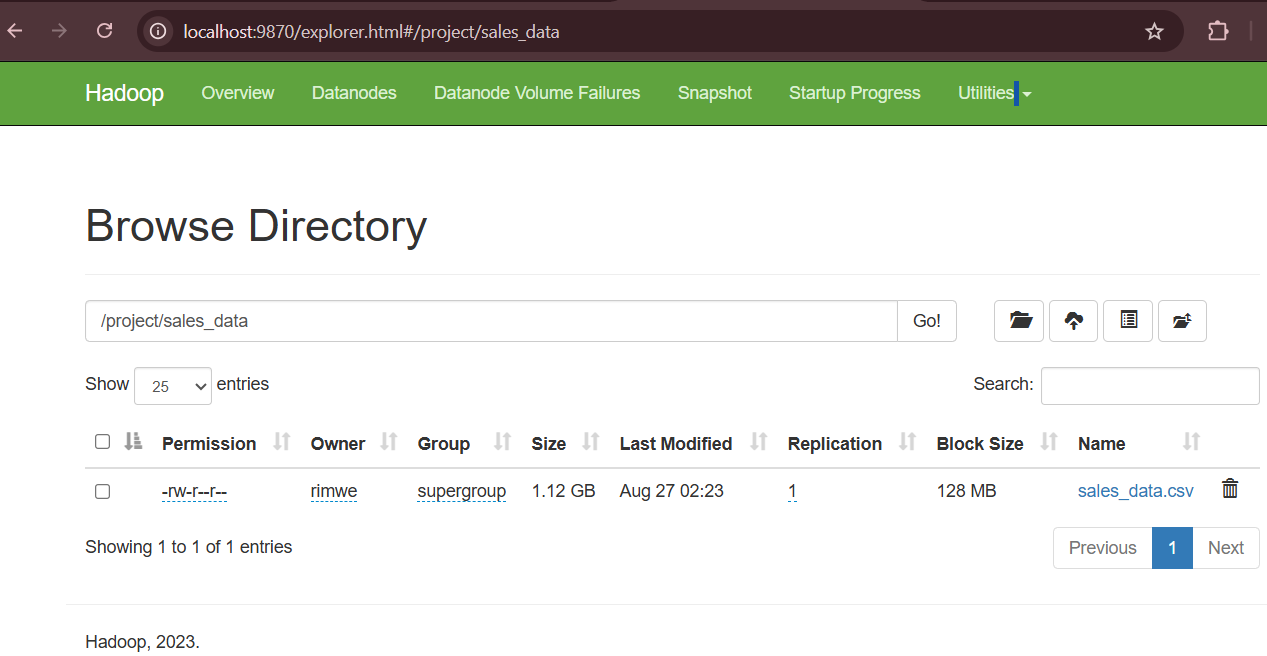
\includegraphics[width=0.9\textwidth]{../screeshots/hdfsbrowser2.png}
    \caption{data loaded in hdfs}
    \label{fig:my-picture}
\end{figure}
\newpage
\begin{figure}[H]
    \centering
    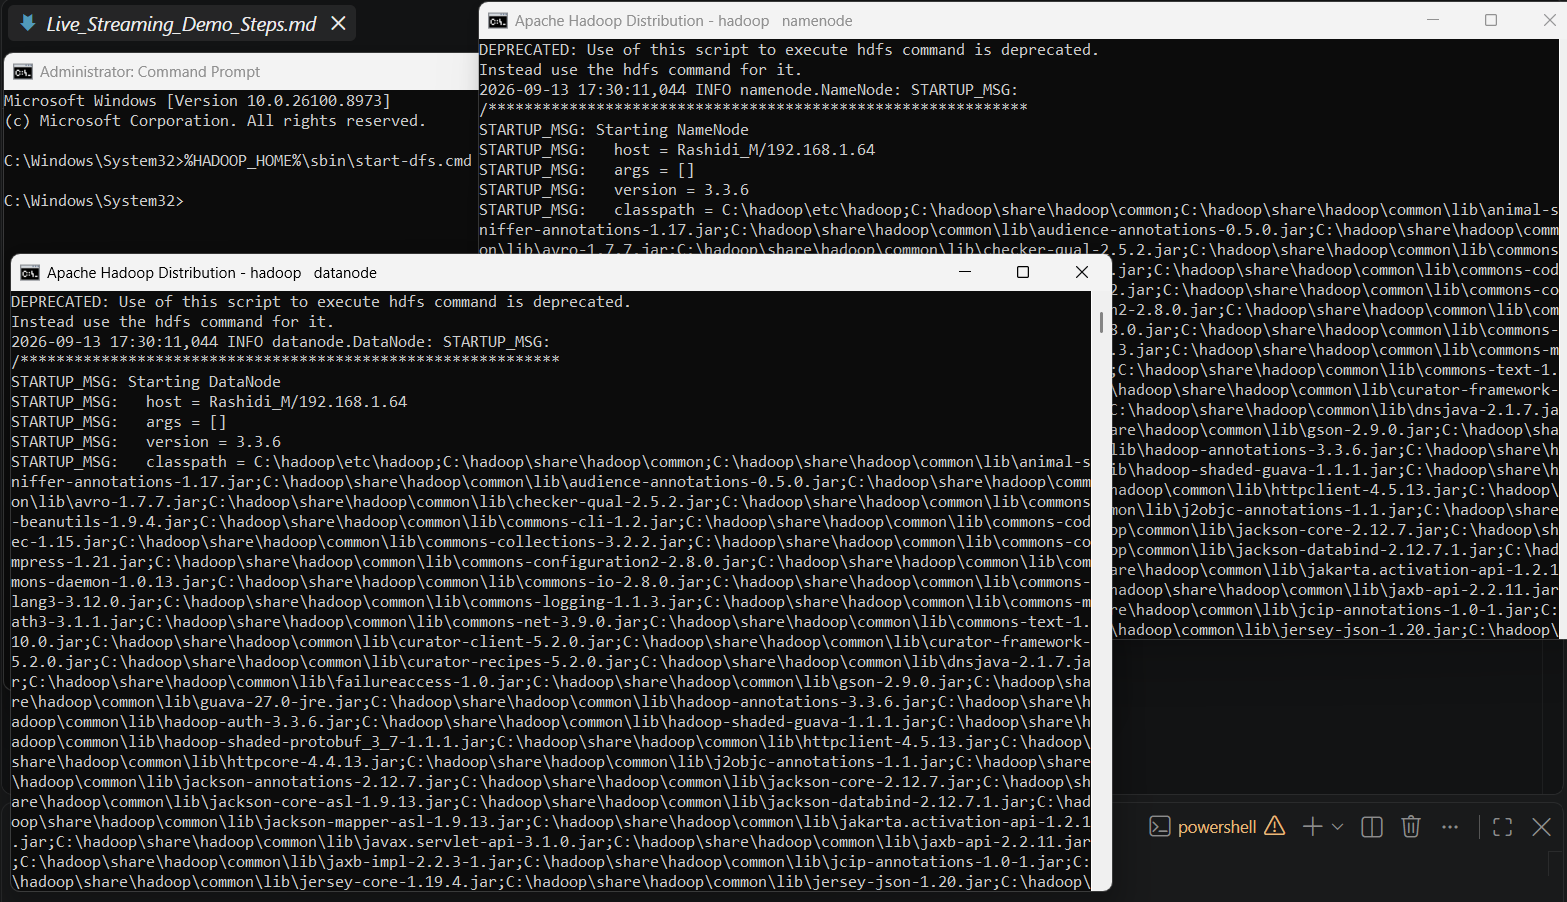
\includegraphics[width=0.9\textwidth]{../screeshots/hdfs.png}
    \caption{apache hadoop distibution}
    \label{fig:my-picture}
\end{figure}

\stephead{2}{Real-Time Data Streaming with Kafka}
A Kafka producer script (\texttt{kafka\_producer.py}) read the dataset from HDFS using PySpark and published each row as a JSON message to a Kafka topic (\texttt{sales-stream}) at a configurable rate, simulating live point-of-sale transactions.

\begin{figure}[H]
    \centering
    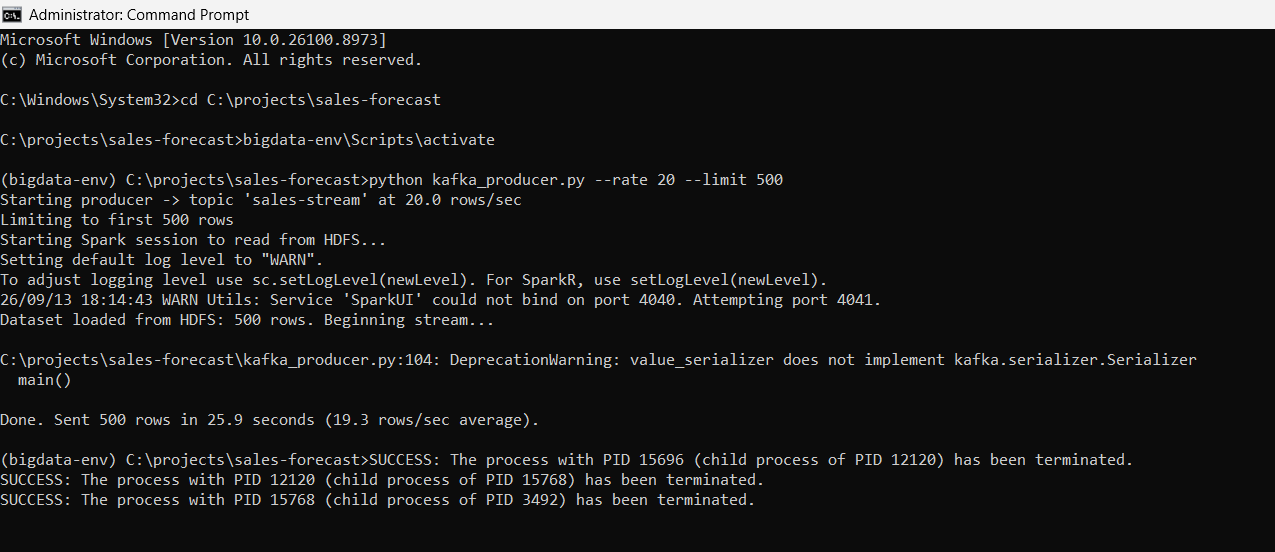
\includegraphics[width=0.9\textwidth]{../screeshots/producer.png}
    \caption{kafka producer}
    \label{fig:my-picture}
\end{figure}
\begin{figure}[H]
    \centering
    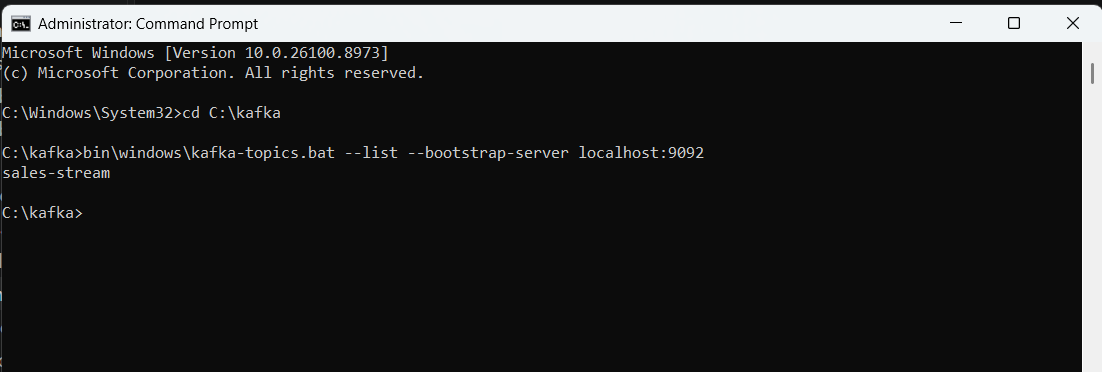
\includegraphics[width=0.9\textwidth]{../screeshots/kafkaStream.png}
    \caption{kafkaStreaming}
    \label{fig:my-picture}
\end{figure}
\begin{figure}[H]
    \centering
    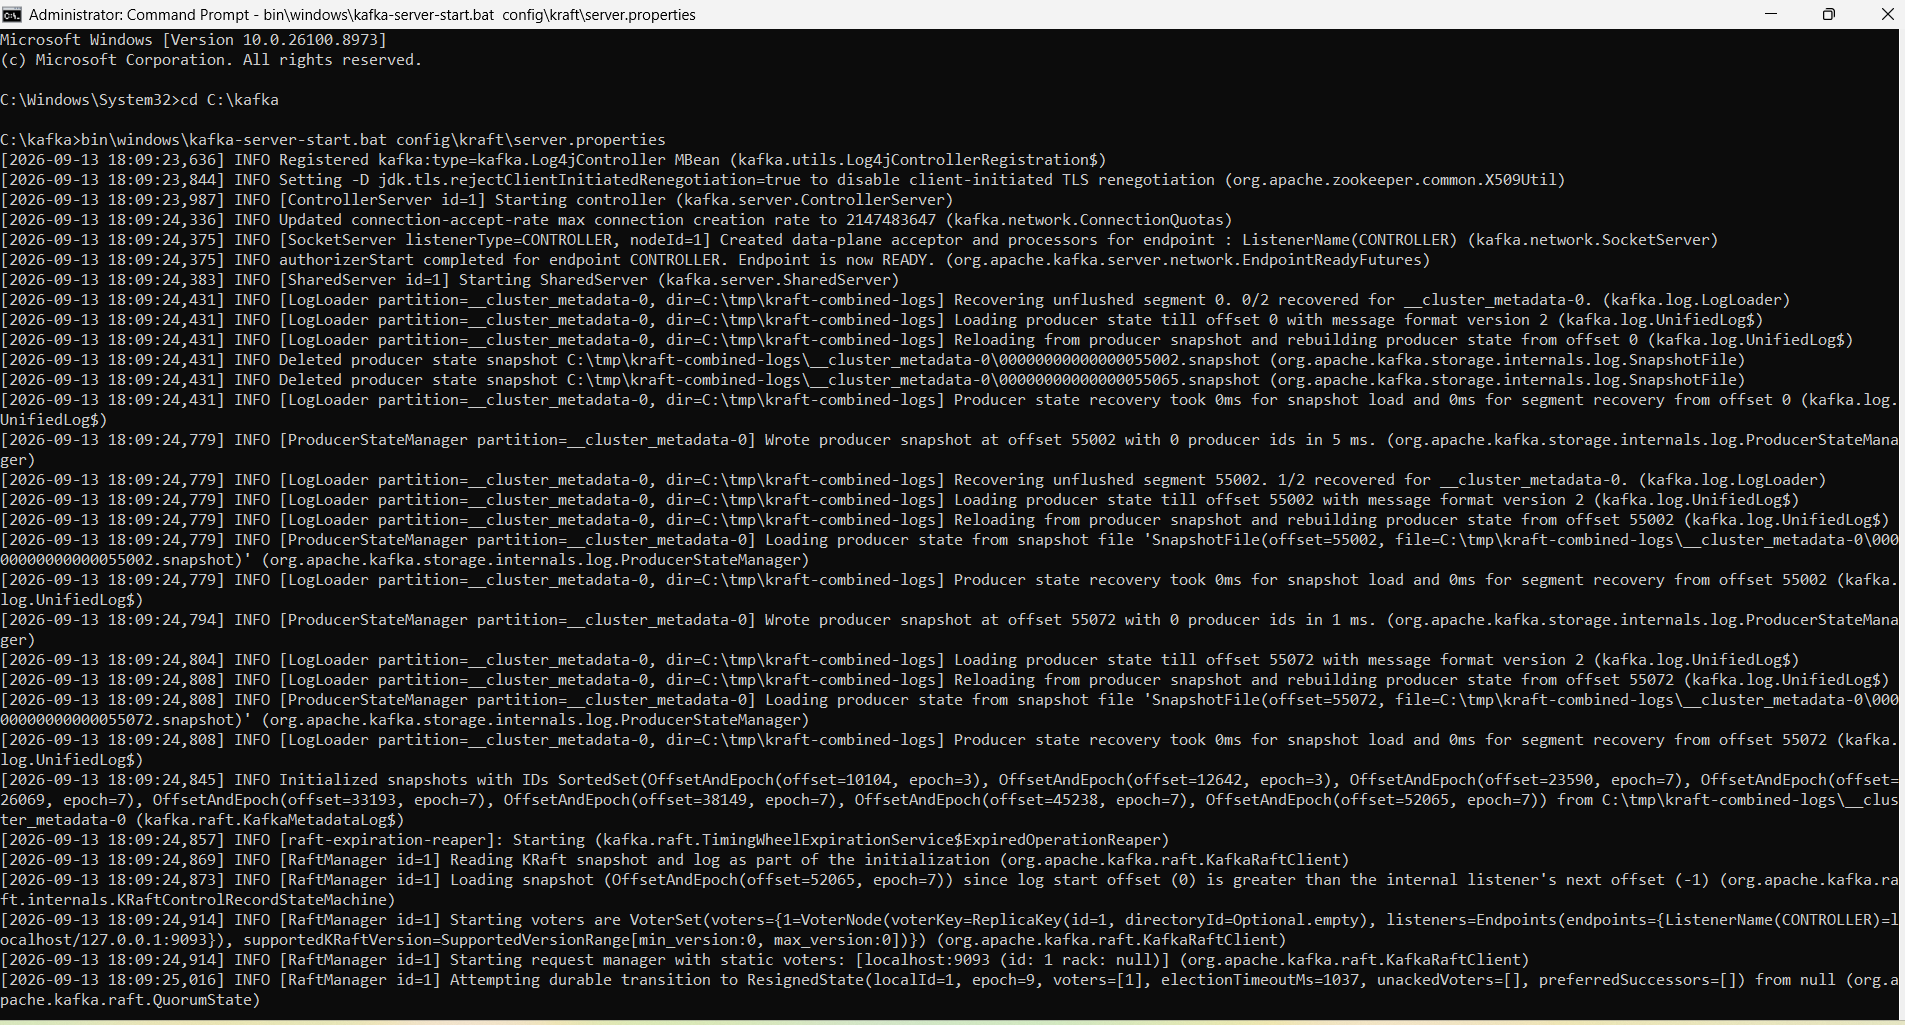
\includegraphics[width=0.9\textwidth]{../screeshots/kafka.png}
    \caption{kafka start}
    \label{fig:my-picture}
\end{figure}

\begin{figure}[H]
    \centering
    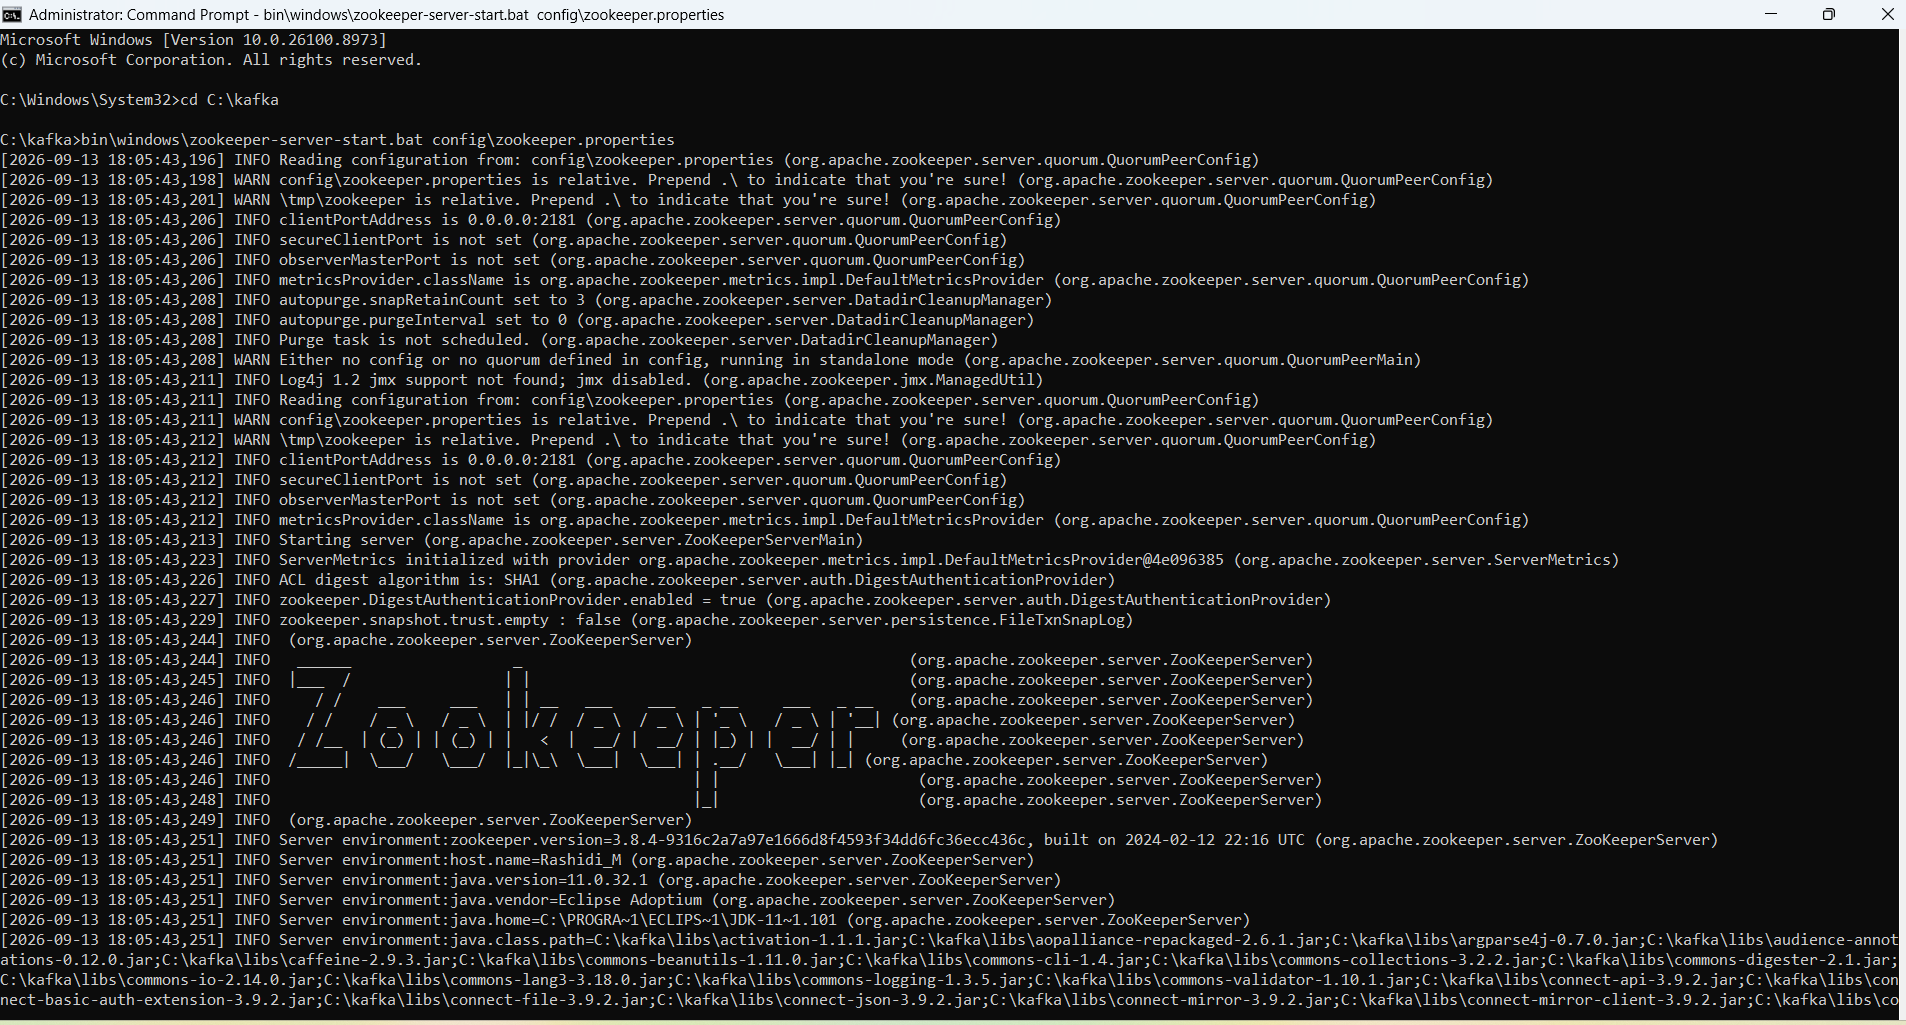
\includegraphics[width=0.9\textwidth]{../screeshots/zookeper.png}
    \caption{zookeeper}
    \label{fig:my-picture}
\end{figure}


\stephead{3}{Data Processing with PySpark}
A PySpark Structured Streaming consumer (\texttt{spark\_streaming\_consumer.py}) subscribed to the Kafka topic, parsed incoming JSON messages against a defined schema, and computed two live views: raw incoming records and running totals of revenue and units sold grouped by region and category.
\begin{figure}[H]
    \centering
    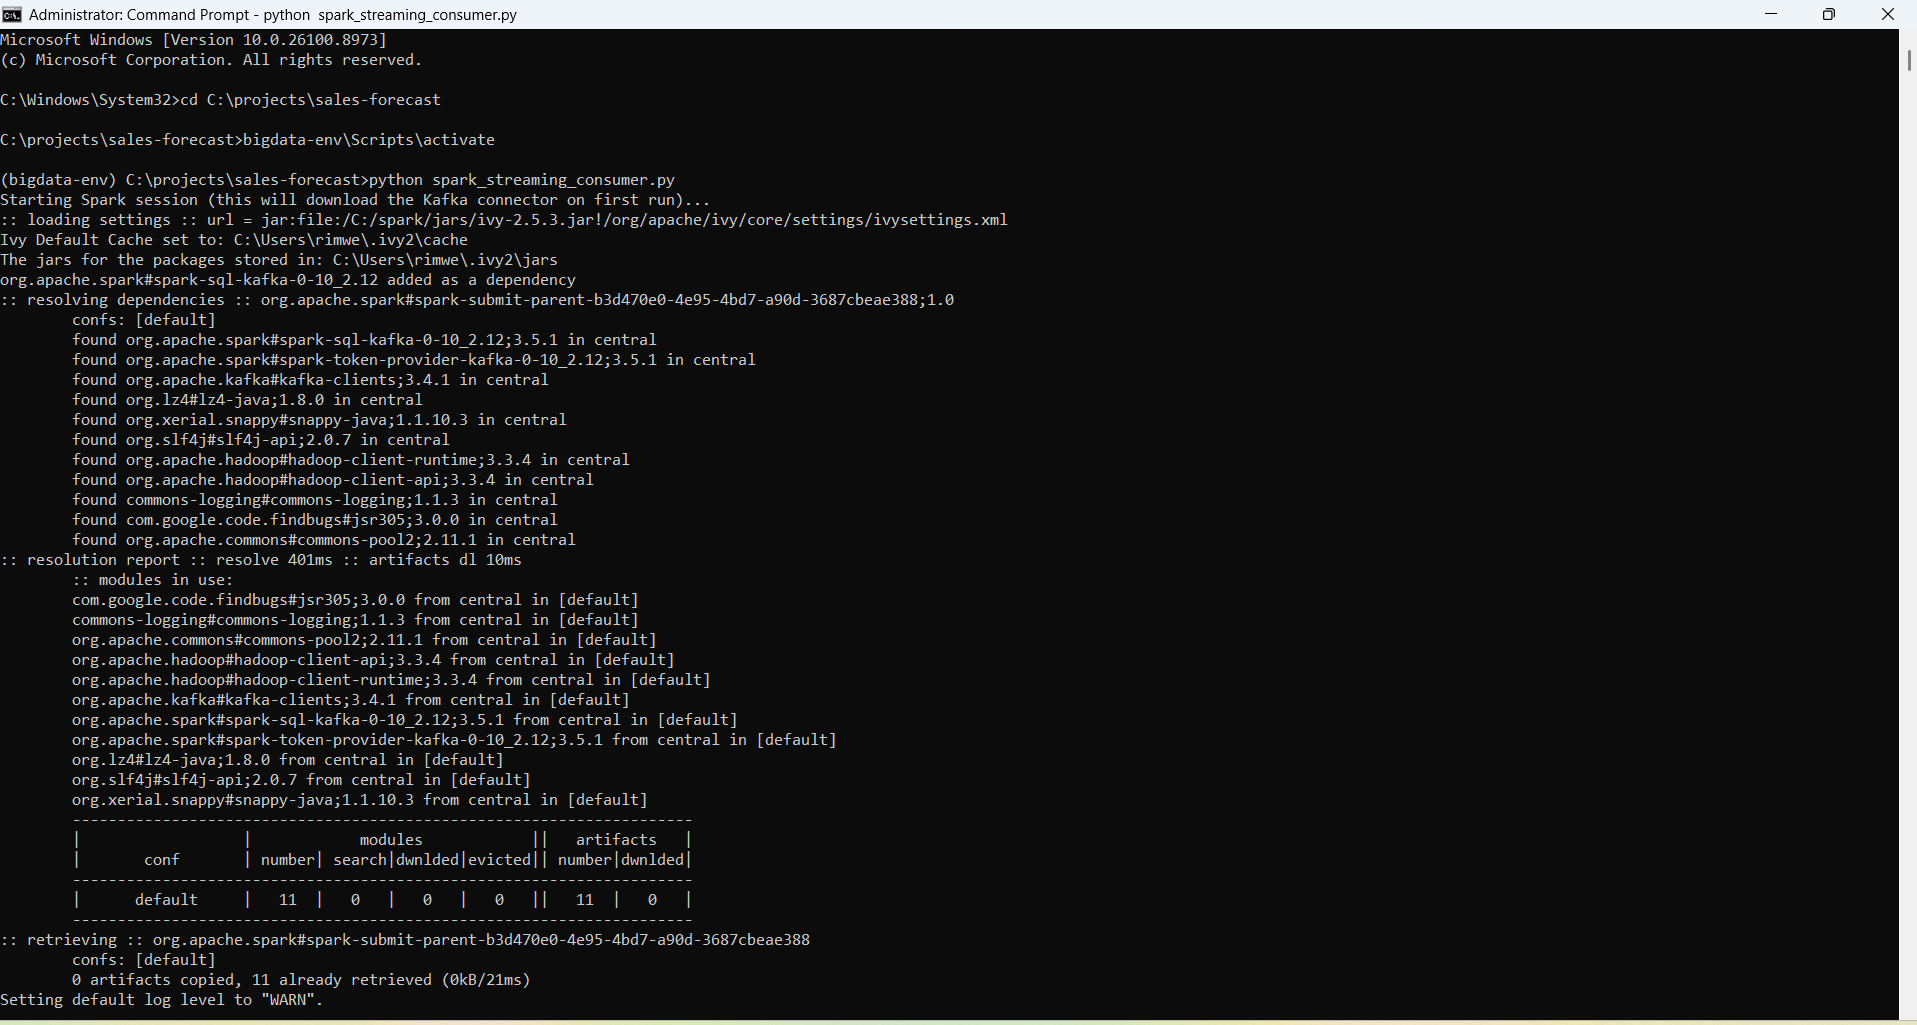
\includegraphics[width=0.9\textwidth]{../screeshots/consumer.png}
    \caption{pyspark streaming consumer}
    \label{fig:my-picture}
\end{figure}

\stephead{4}{Prediction Modeling with MLlib}
A separate batch script (\texttt{train\_and\_predict.py}) read the full historical dataset from HDFS, aggregated it to daily revenue totals, engineered ten features (day of week, month, weekend flag, holiday-season flag, promotion rate, average discount, transaction count, units sold, previous-day revenue, and a 7-day rolling average revenue), and trained a Random Forest Regressor using a time-based 1,645/180-day train/test split.
\begin{figure}[H]
    \centering
    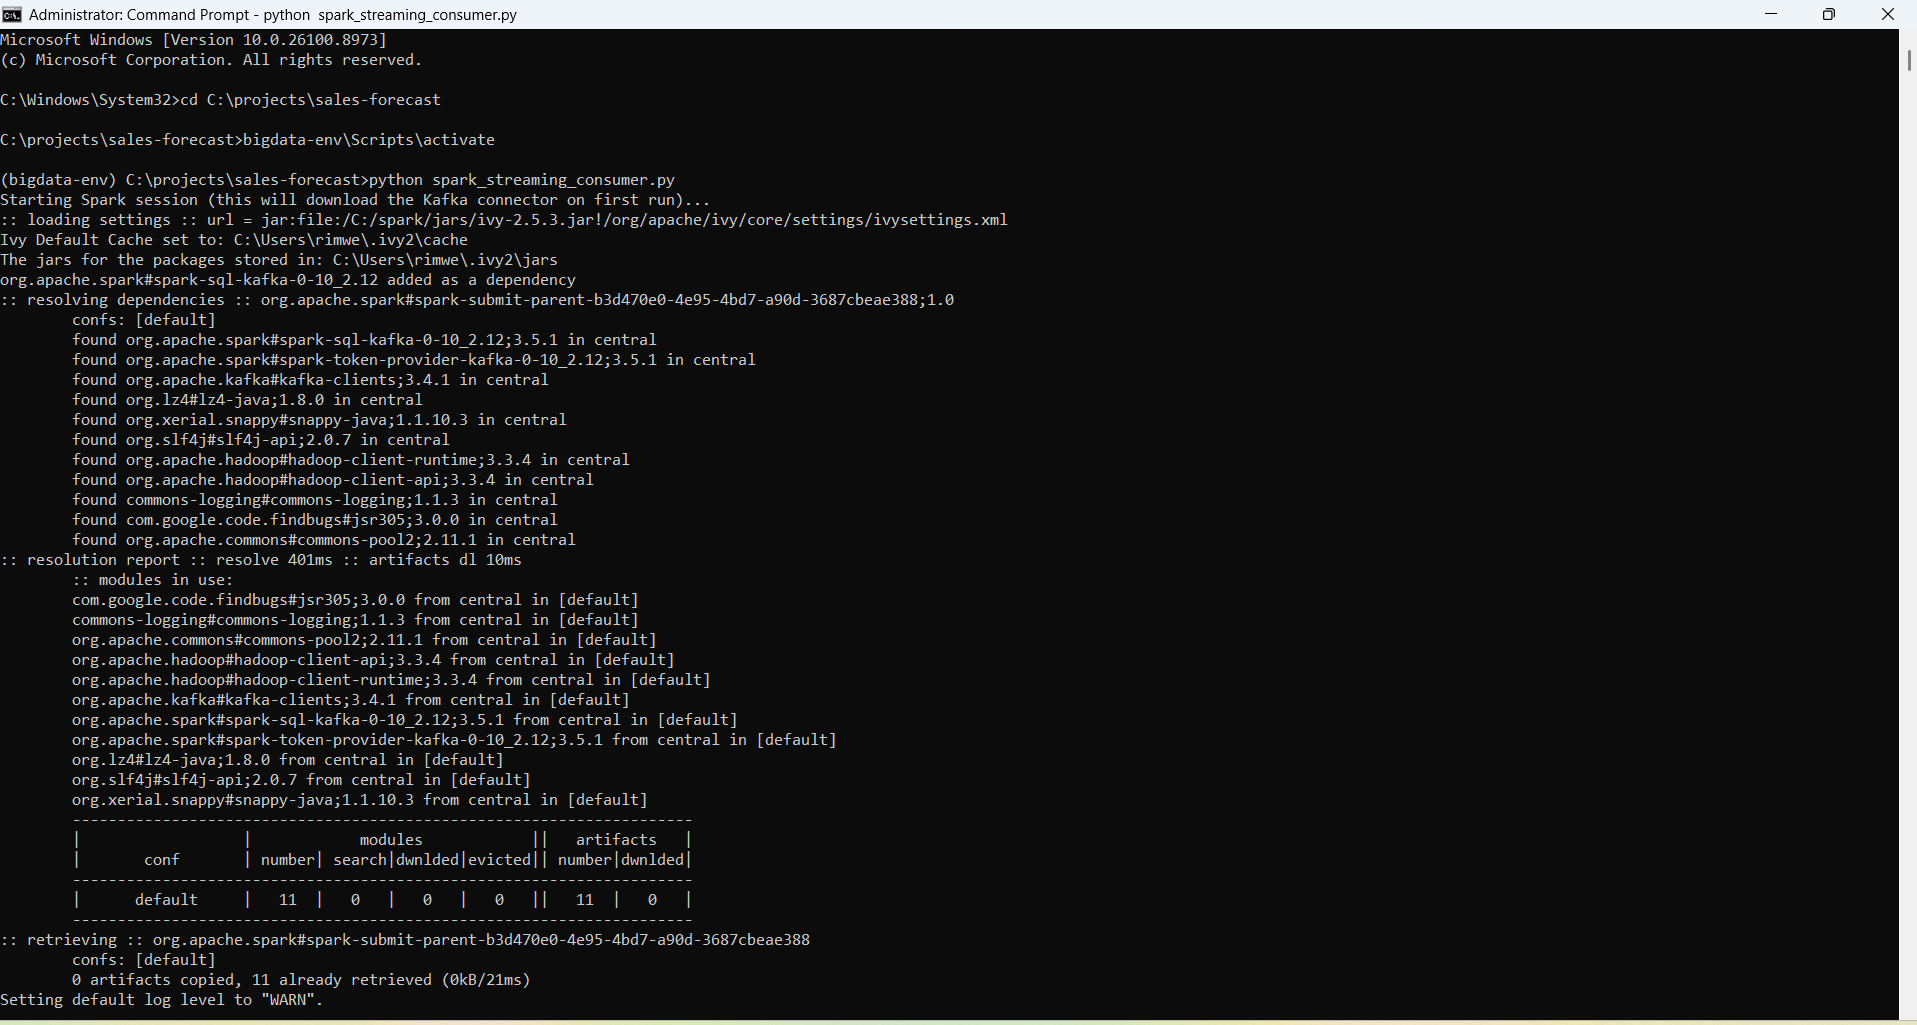
\includegraphics[width=0.9\textwidth]{../screeshots/consumer.png}
    \caption{pyspark streaming consumer}
    \label{fig:my-picture}
\end{figure}
\stephead{5}{Store Data and Predictions in MySQL}
Model predictions on the held-out test period were written to a MySQL table (\texttt{daily\allowbreak\_sales\allowbreak\_predictions}) via Spark's JDBC writer. The streaming consumer separately wrote live aggregates (\texttt{live\allowbreak\_region\allowbreak\_category\allowbreak\_totals}) and a rolling transaction feed (\texttt{live\allowbreak\_recent\allowbreak\_transactions}) to MySQL using a \texttt{foreachBatch} sink.

\begin{figure}[H]
    \centering
    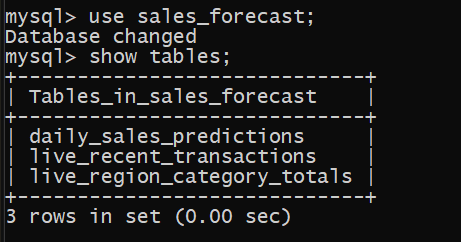
\includegraphics[width=6cm,height=4cm]{../screeshots/database.png}
    \caption{Database and tables}
    \label{fig:my-picture}
\end{figure}
\begin{figure}[H]
    \centering
    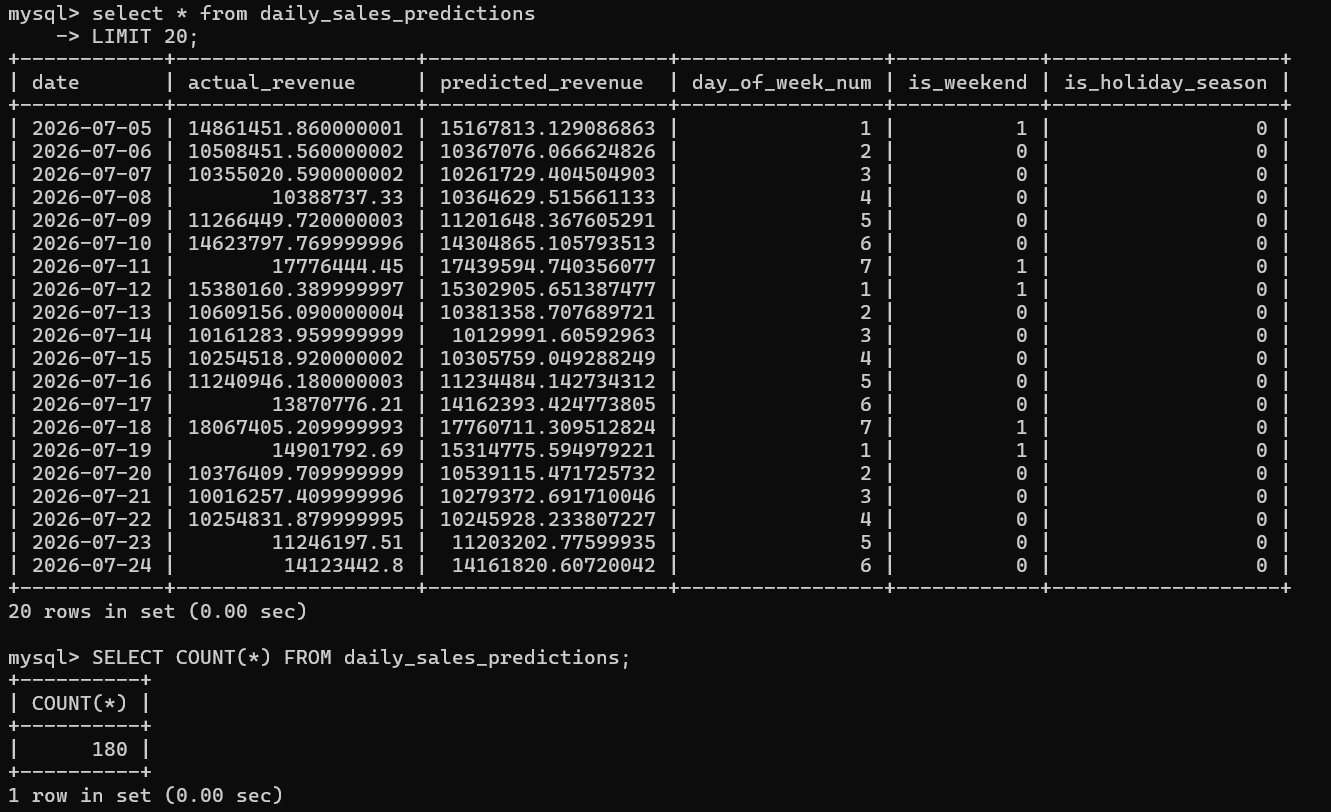
\includegraphics[width=0.9\textwidth]{../screeshots/daily_sales_predictions.png}
    \caption{daily sales predictions}
    \label{fig:my-picture}
\end{figure}
\begin{figure}[H]
    \centering
    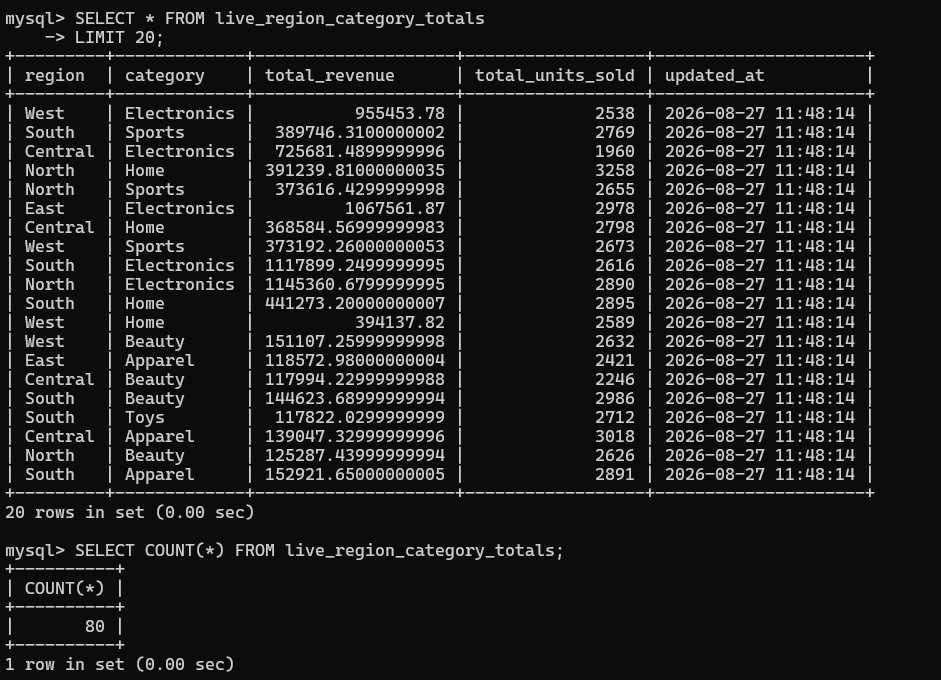
\includegraphics[width=15cm,height=10cm]{../screeshots/live_region_category_totals.png}
    \caption{live region category totals}
    \label{fig:my-picture}
\end{figure}
\begin{figure}[H]
    \centering
    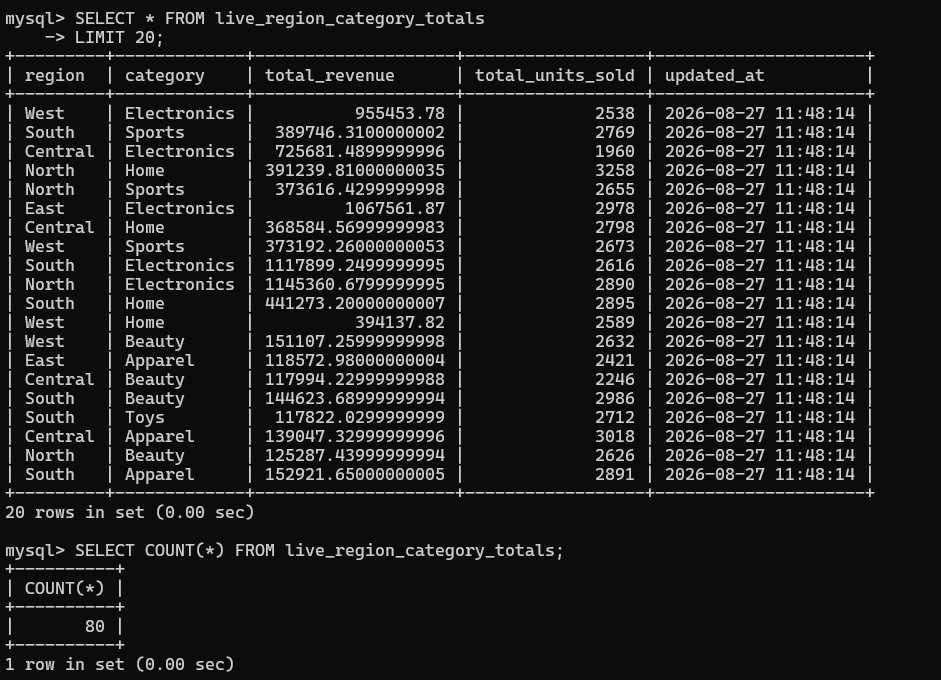
\includegraphics[width=15cm,height=10cm]{../screeshots/live_region_category_totals.png}
    \caption{live region category totals}
    \label{fig:my-picture}
\end{figure}


\stephead{6}{Build a Django Web Dashboard}
A Django application was built with four pages Overview, Predictions, Charts, and Live all reading from the MySQL database using the \texttt{mysql-connector-python} Django backend. The Live page polls a JSON API endpoint every 2.5 seconds to reflect new streaming data without a page reload.

\begin{figure}[H]
    \centering
    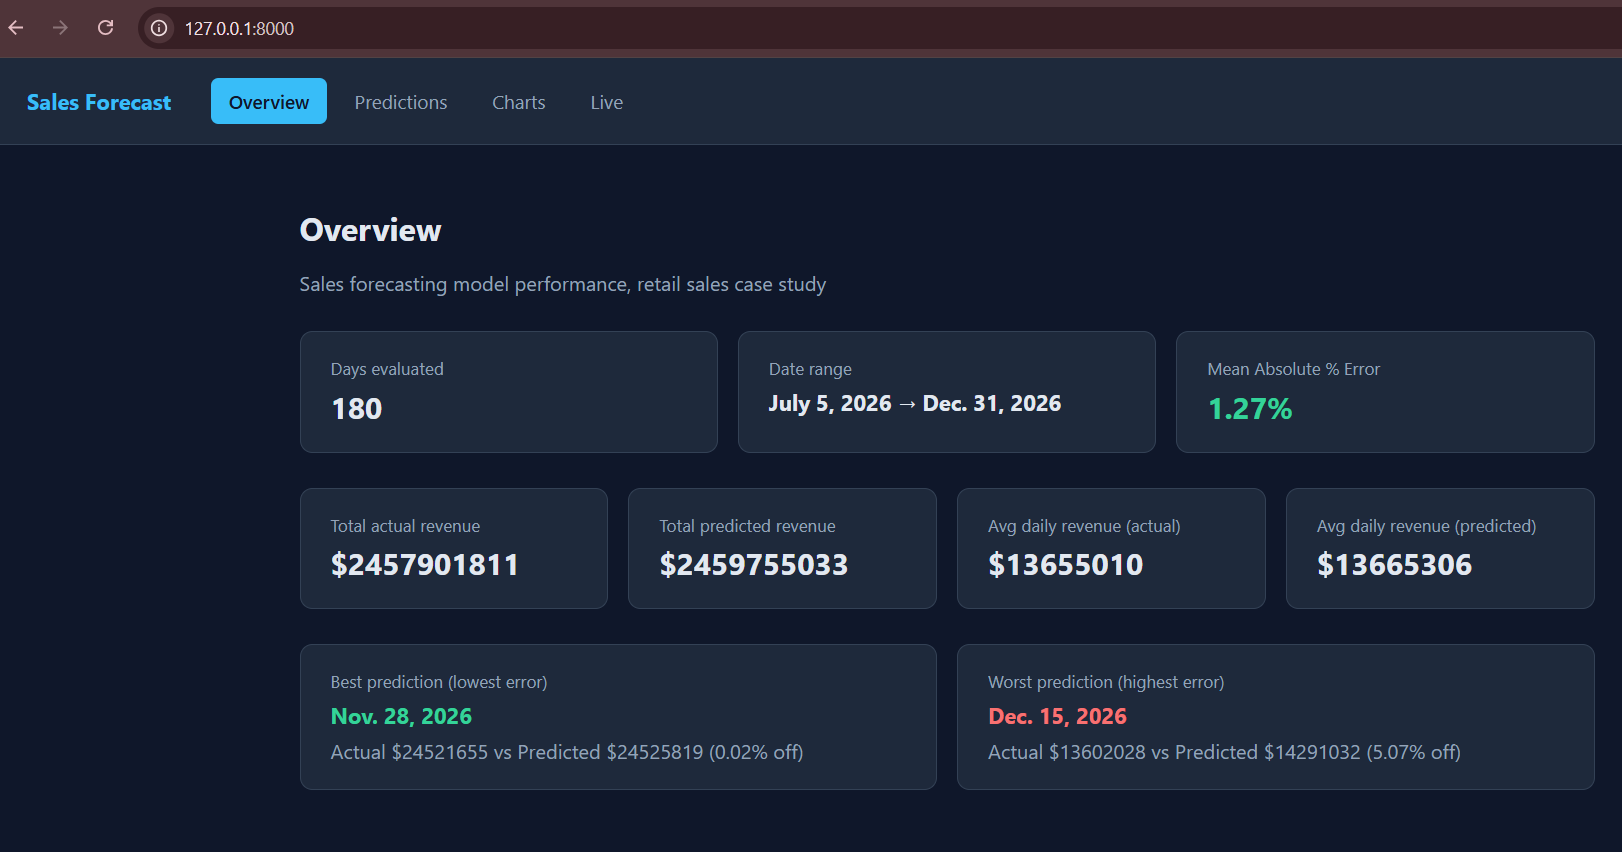
\includegraphics[width=15cm,height=7cm]{../screeshots/overview.png}
    \caption{Django webdashboard}
    \label{fig:my-dashboard}
\end{figure}
\begin{figure}[H]
    \centering
    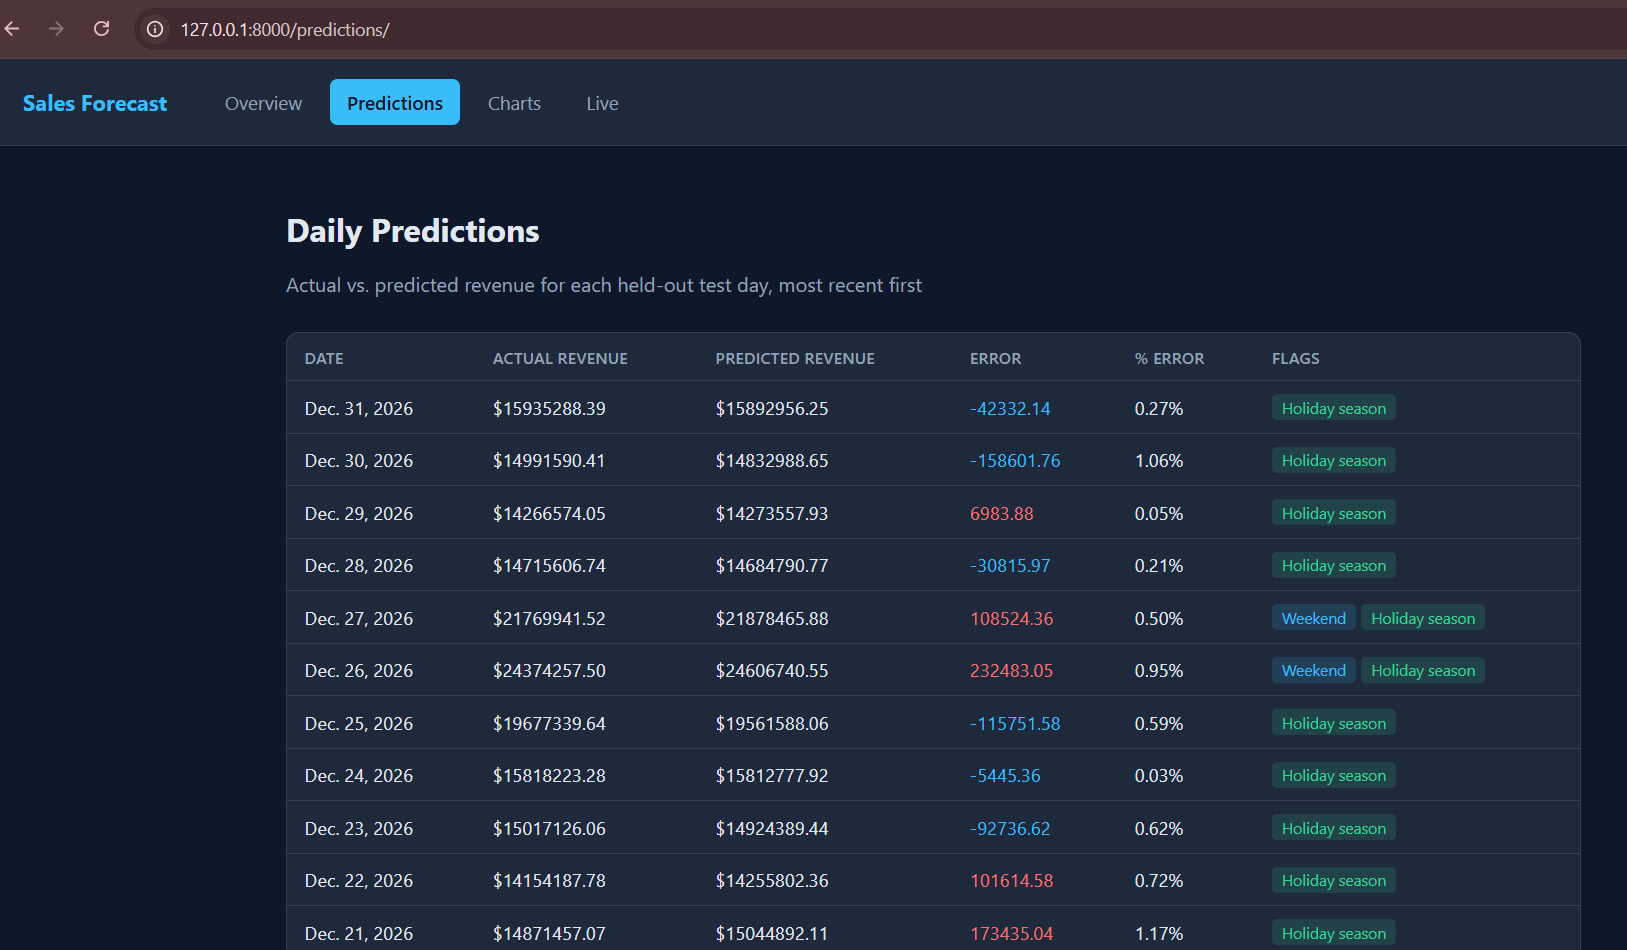
\includegraphics[width=15cm,height=6cm]{../screeshots/predictions.png}
    \caption{predictions on the web page}
    \label{fig:my-predictions}
\end{figure}
\begin{figure}[H]
    \centering
    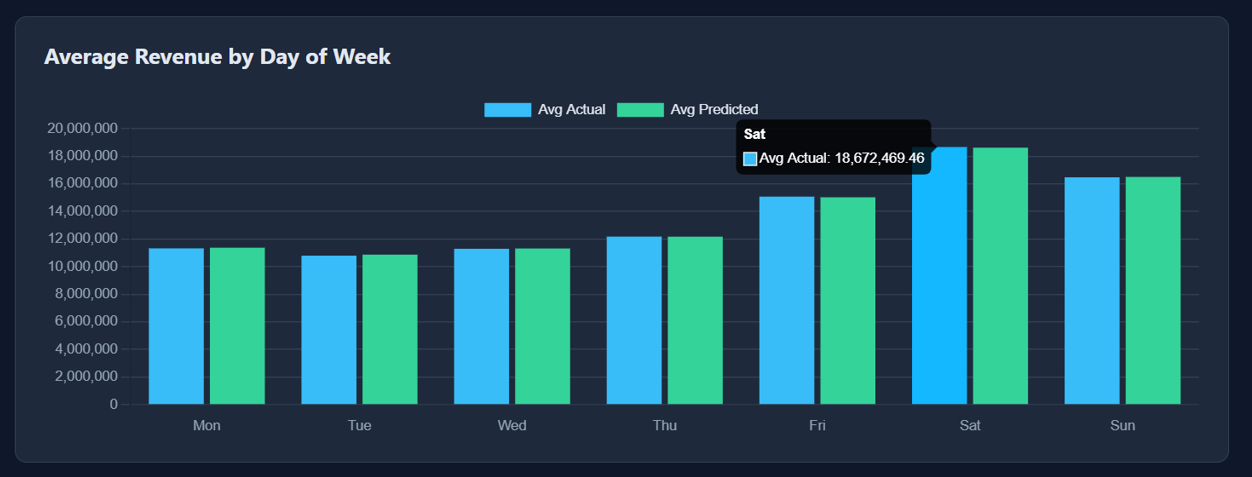
\includegraphics[width=15cm,height=6cm]{../screeshots/average_revenue_by_week.png}
    \caption{average revenue by week}
    \label{fig:my-paverage}
\end{figure}
\begin{figure}[H]
    \centering
    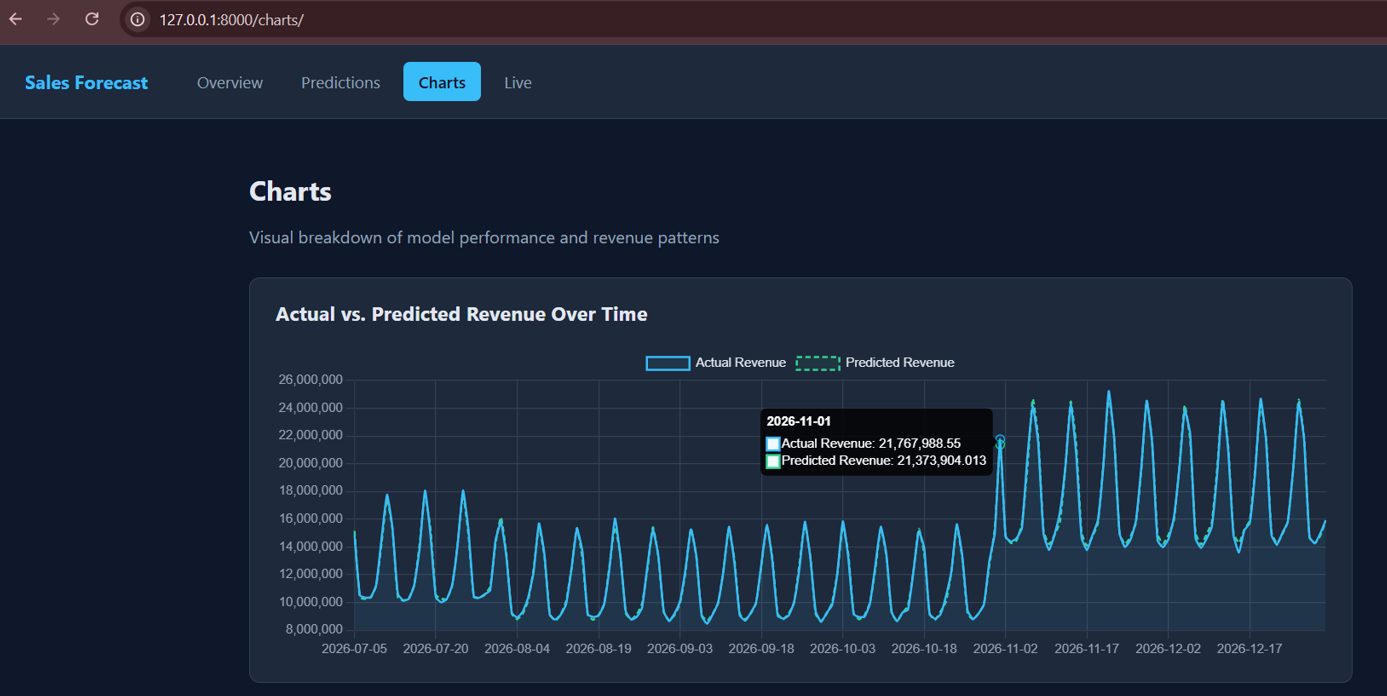
\includegraphics[width=15cm,height=6cm]{../screeshots/actual_and_predicted_revenue.png}
    \caption{actual vs predicted revenue}
    \label{fig:my-pactual}
\end{figure}
\begin{figure}[H]
    \centering
    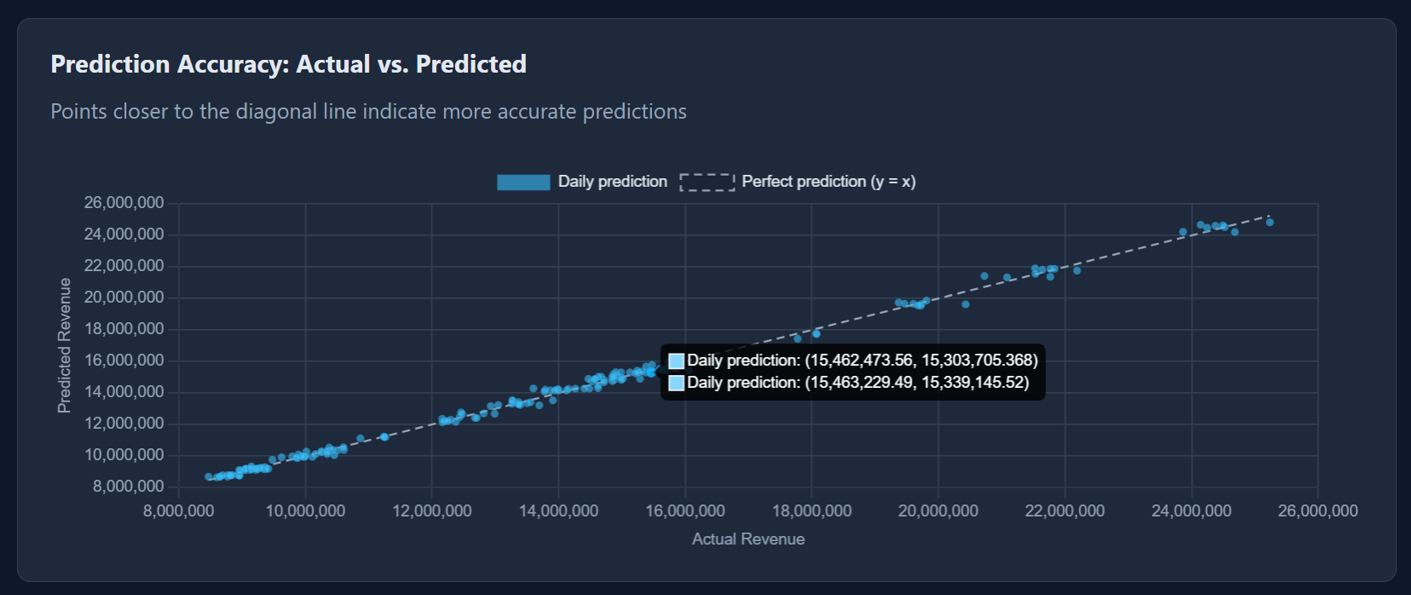
\includegraphics[width=15cm,height=6cm]{../screeshots/prediction_accuracy.png}
    \caption{prediction accuracy}
    \label{fig:my-pacl}
\end{figure}
\begin{figure}[H]
    \centering
    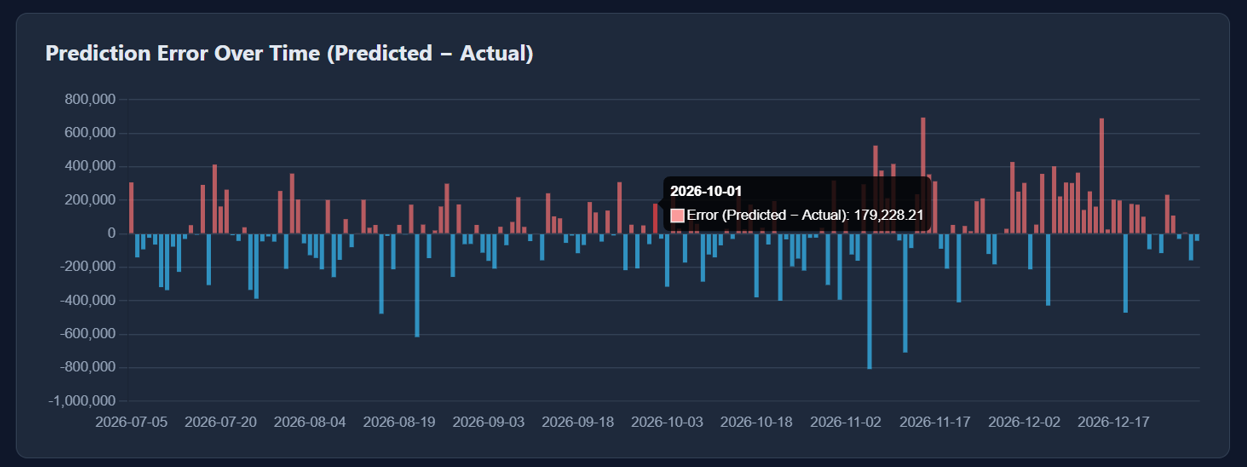
\includegraphics[width=15cm,height=6cm]{../screeshots/prediction_error.png}
    \caption{prediction error}
    \label{fig:my-pach}
\end{figure}
\begin{figure}[H]
    \centering
    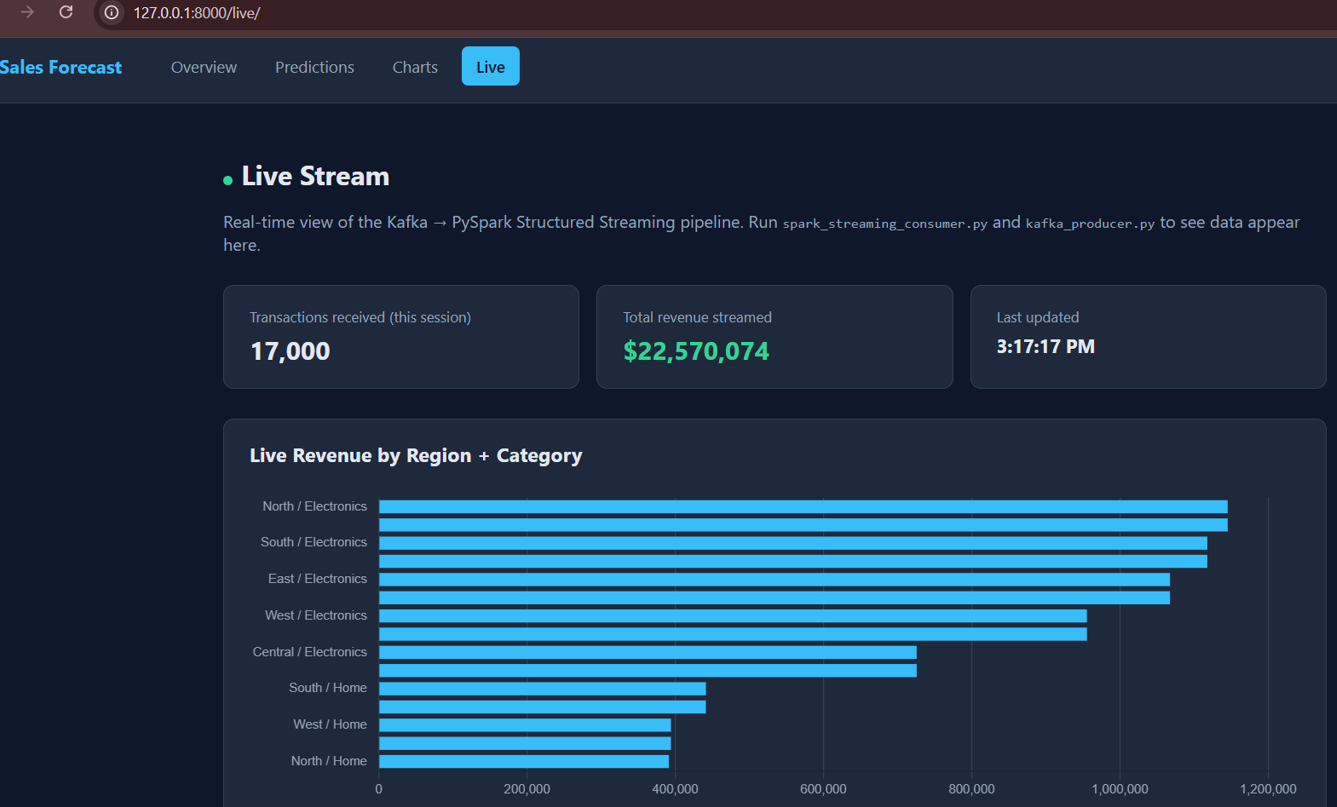
\includegraphics[width=15cm,height=7cm]{../screeshots/live-stream.png}
    \caption{Live streaming dashboard}
    \label{fig:my-live-streaming}
\end{figure}
\stephead{7}{Testing and Deployment}
Each pipeline component was verified independently (HDFS file listing, Kafka topic creation and message delivery, Spark shell startup, MySQL connectivity) before being connected end to end. The full pipeline was run together and verified via a live demonstration: starting HDFS, Kafka, and MySQL, running the streaming consumer and producer concurrently, and confirming that the Django dashboard reflected new data within seconds.

% ==================== 6. FINDINGS ====================
\section{Findings}

\subsection{Model Performance}

The Random Forest Regressor (100 trees, maximum depth 8) was evaluated on a held-out set of the most recent 180 days of daily revenue, following a time-based (not random) train/test split appropriate for forecasting tasks.

\begin{table}[H]
\centering
\begin{tabularx}{\textwidth}{@{}>{\raggedright\arraybackslash}p{2.3cm}>{\raggedright\arraybackslash}p{2.6cm}>{\raggedright\arraybackslash}X@{}}
\toprule
\rowcolor{navy}\textcolor{white}{\textbf{Metric}} & \textcolor{white}{\textbf{Value}} & \textcolor{white}{\textbf{Interpretation}} \\
\midrule
RMSE & 233{,}398.14 & Average magnitude of prediction error, in revenue currency units \\
\rowcolor{rowalt} MAE & 177{,}179.90 & Average absolute prediction error \\
R\textsuperscript{2} & 0.9969 & The model explains 99.69\% of the variance in daily revenue \\
\bottomrule
\end{tabularx}
\end{table}

\subsection{Feature Importance}

The trained model's feature importances reveal which factors most strongly drive daily revenue predictions:

\begin{table}[H]
\centering
\begin{tabularx}{0.85\textwidth}{@{}>{\raggedright\arraybackslash}Xr@{}}
\toprule
\rowcolor{navy}\textcolor{white}{\textbf{Feature}} & \textcolor{white}{\textbf{Importance}} \\
\midrule
daily\_units\_sold & \textbf{0.5067} \\
\rowcolor{rowalt} month\_num & 0.1168 \\
is\_weekend & 0.1168 \\
\rowcolor{rowalt} is\_holiday\_season & 0.1044 \\
day\_of\_week\_num & 0.0803 \\
\rowcolor{rowalt} prev\_day\_revenue & 0.0488 \\
rolling\_7day\_avg\_revenue & 0.0224 \\
\rowcolor{rowalt} transaction\_count & 0.0022 \\
avg\_discount\_pct & 0.0010 \\
\rowcolor{rowalt} promo\_rate & 0.0008 \\
\bottomrule
\end{tabularx}
\end{table}

\subsection{Discussion}

\begin{itemize}[leftmargin=1.4em, itemsep=3pt]
    \item Units sold is by far the dominant predictor (50.7\% importance), which is expected since revenue is mechanically driven by volume this confirms the model has correctly learned the core relationship in the data.
    \item Calendar-based seasonality (month, weekend, and holiday-season flags) collectively account for roughly a third of the model's predictive power, validating the deliberate weekday and holiday-season effects built into the synthetic dataset.
    \item The lag-based features (previous-day revenue and the 7-day rolling average) contribute modestly but meaningfully, indicating short-term revenue momentum carries some forecasting value beyond same-day attributes alone.
    \item Promotion-related fields (\texttt{promo\_rate}, \texttt{avg\_discount\_pct}) show minimal standalone importance, likely because their effect is already captured indirectly through \texttt{daily\_units\_sold}, since promotions in the dataset primarily act by boosting the units-sold figure.
    \item The very high R\textsuperscript{2} (0.9969) reflects both a genuinely learnable underlying pattern and the fact that the daily aggregation smooths out much of the transaction-level noise present in the raw 17.5-million-row dataset.
\end{itemize}

\subsection{Scale Summary}

\begin{table}[H]
\centering
\begin{tabularx}{0.85\textwidth}{@{}>{\raggedright\arraybackslash}Xr@{}}
\toprule
\rowcolor{navy}\textcolor{white}{\textbf{Item}} & \textcolor{white}{\textbf{Value}} \\
\midrule
Raw transaction records & 17,500,000 rows \\
\rowcolor{rowalt} Raw dataset size in HDFS & 1.12 GB \\
Aggregated daily records & 1,825 days (2022-2026) \\
\rowcolor{rowalt} Training set & 1,645 days \\
Test set (held out) & 180 days (most recent) \\
\rowcolor{rowalt} Kafka topic partitions & 1 (single-node development setup) \\
\bottomrule
\end{tabularx}
\end{table}
\renewcommand{\arraystretch}{1}

% ==================== 7. CONCLUSION ====================
\section{Conclusion}

This project successfully demonstrates a complete, working Big Data pipeline that spans distributed storage, real-time streaming, distributed processing, machine learning, relational persistence, and web-based visualization. Every component HDFS, Kafka, PySpark (both batch and Structured Streaming), Spark MLlib, MySQL, and Django was integrated and verified end to end on a Windows development environment, including a live-updating dashboard that reflects the real-time streaming pipeline within seconds. The trained Random Forest model achieved strong predictive accuracy (R\textsuperscript{2} = 0.9969) on held-out data, and its feature importances offer genuine, interpretable insight into the drivers of daily retail revenue.

% ==================== 8. APPENDIX ====================
\section{Appendix: Project Files}

\renewcommand{\arraystretch}{1.25}
\begin{table}[H]
\centering
\begin{tabularx}{\textwidth}{@{}>{\raggedright\arraybackslash}p{5.4cm}>{\raggedright\arraybackslash}X@{}}
\toprule
\rowcolor{navy}\textcolor{white}{\textbf{File}} & \textcolor{white}{\textbf{Purpose}} \\
\midrule
\texttt{generate\_sales\_data.py} & Synthetic dataset generator \\
\rowcolor{rowalt} \texttt{kafka\_producer.py} & Reads HDFS data and streams it into Kafka \\
\texttt{spark\_streaming\_consumer.py} & PySpark Structured Streaming consumer; writes live data to MySQL \\
\rowcolor{rowalt} \texttt{train\_and\_predict.py} & Batch feature engineering, MLlib model training, and prediction storage \\
\texttt{sales\_dashboard/} (Django project) & Web dashboard: Overview, Predictions, Charts, Live pages \\
\bottomrule
\end{tabularx}
\end{table}
\renewcommand{\arraystretch}{1}

\end{document}
